\documentclass[conference]{IEEEtran}
\usepackage[T1]{fontenc}
\usepackage{amsmath,amssymb,booktabs,array,graphicx}
\usepackage{algorithm,algpseudocode}
\usepackage{tikz}
\usetikzlibrary{arrows.meta,positioning,fit}
\usepackage[hidelinks]{hyperref}
\usepackage{url}
\usepackage{cite}
\usepackage{balance}
\graphicspath{{figures/}}
\newcommand{\Yes}{\mathsf{true}}
\newcommand{\No}{\mathsf{false}}
\newcommand{\Cset}{C(E)}
\newcommand{\code}[1]{\texttt{#1}}
\newcommand{\pp}{\,pp}
\newtheorem{proposition}{Proposition}
\pagestyle{plain}
\title{When Is Evidence Enough?\\Checkable Contracts for Bounded Agent Workflows}
\author{\IEEEauthorblockN{Victor Cao}
\IEEEauthorblockA{University of Auckland\\Auckland, New Zealand\\xcao541@aucklanduni.ac.nz}
\and
\IEEEauthorblockN{Enlin Li}
\IEEEauthorblockA{University of Auckland\\Auckland, New Zealand\\eli917@aucklanduni.ac.nz}}

\begin{document}
\maketitle
\thispagestyle{plain}
\begin{abstract}
An agent may have permission to act without enough evidence that its task will succeed. A lost reply creates another uncertainty: an action may already have taken effect. We study these problems through checkable evidence contracts in a bounded synthetic workflow language. A query selector gathers trusted observations and execution receipts. A separate checker permits a fixed route only when the evidence covers every world still consistent with the observations. A recovery controller distinguishes confirmed commits, fenced noncommits, and unresolved outcomes. We evaluate 36 structural families, 1,006 reference-checked executions, and 288 live model-selection streams. Certificate stopping reduces mean queries from 7.750 to 3.014 while preserving 81.94\% family-mean completion. On 36 matched model tasks, a deterministic selector completes 30, compared with 29 and 28 for the two models. Graph information shows no stable advantage over a padding control. Recovery improves acknowledged completion, but part of that gain confirms work already completed. The study provides executable evidence, counterexamples, and reproducible negative results. Its claims depend on finite world coverage and trusted execution records; they do not establish protection for real Skills or unrestricted agents.
\end{abstract}
\begin{IEEEkeywords}
LLM agents, evidence contracts, active information gathering, runtime enforcement, fault recovery, reproducibility
\end{IEEEkeywords}

\section{Introduction}
\label{sec:intro}
Large language model (LLM) agents can read files, call tools, and change external state. Agent Skills extend this behaviour with reusable instructions, scripts, and supporting resources. This makes Skills useful, but also creates several places where untrusted content can influence an action. Studies of malicious Skills and indirect prompt injection show why the source and purpose of an instruction matter \cite{liu,skillinject,injecagent}. A useful defence must therefore control effects as well as inspect text.

Permission alone does not establish that a task will succeed. Consider an agent that is allowed to write a report and emit a completion message. It may still choose a route that reads the wrong input, fails before writing, or produces the wrong output. Blocking every uncertain route avoids some mistakes, but also prevents useful work. The practical question is how much evidence is enough to allow a particular route to run.

Execution introduces a second question: what should the agent do when a reply is lost? A write may already have committed even though the controller sees an error. Retrying can duplicate the effect, while stopping can leave a task incomplete. A missing status record does not settle this problem because the original request may still be pending. Safe continuation needs evidence about the operation's state, rather than another guess about its outcome.

These questions are related but distinct. Authorization asks whether an effect is permitted. Task certification asks whether one route will complete the goal under the states that remain possible. Recovery asks whether a previous effect committed and whether a new attempt is safe. Combining all three into a single ``safe'', ``unsafe'', or ``unknown'' label hides the reason for a decision. It also makes a failure difficult to interpret: the problem might be missing information, an impossible fixed-route requirement, or an unresolved operation.

Our earlier literature review proposed generating task-conditioned capability policies from user requests and Skill content. The completed study has a narrower scope. We take the task goal, candidate programs, world catalog, and permissions as explicit inputs. We then study how evidence supports execution and recovery within that fixed interface. This change is necessary because policy generation, open-ended code analysis, and execution uncertainty cannot all be validated by the same small experiment. The present paper does not claim to have solved the original policy-generation problem.

The resulting system separates evidence selection from evidence checking. A selector chooses which query to acquire next. It may be a deterministic heuristic or an LLM. The query service returns an observation or an execution receipt. A separate checker accepts a route only when the required evidence is present. The selector cannot create permissions, invent a receipt, or replace the route catalog. This separation lets us compare selectors without changing the condition for execution.

The study addresses four research questions:
\begin{enumerate}
\item \textbf{RQ1: Sufficient evidence.} Can certificate-based stopping reduce acquired work while preserving completion within the stated contract?
\item \textbf{RQ2: Remaining uncertainty.} Which unknown outcomes could be resolved by better acquisition, and which reflect the limits of the permitted observations and fixed routes?
\item \textbf{RQ3: Selection and representation.} Do model-selected queries or a source-derived graph improve completion or acquisition cost over a capable deterministic selector?
\item \textbf{RQ4: Legal recovery.} Which commit-status records support continuation after an ambiguous result, and which require abstention?
\end{enumerate}

We test corresponding expectations. First, stopping after a valid certificate should preserve the certified route's validity while avoiding later queries. Second, more queries cannot always resolve uncertainty: indistinguishable worlds may require different routes. Third, if a graph provides a useful representation advantage, that advantage should survive a control with similar input length. Finally, terminal commit evidence should support recovery, while an absent or pending record should not. These expectations concern a finite executable model. They are not claims about all LLM agents.

The paper makes three contributions. First, it gives an explicit evidence contract with positive, negative, and unresolved outcomes, together with short soundness arguments and executable counterexamples. Second, it evaluates acquisition, stopping, and recovery using a separate reference implementation and controlled synthetic families. Third, it reports the limits of the approach through strong comparisons, retained failures, and a distinction between acknowledged completion and physical progress. The results include negative findings: neither tested model beats the main heuristic, and graph effects are not stable against the padding control.

The empirical scope is deliberately bounded. The combined benchmark contains 72 cases from 36 structural families; lexical variants and repeated conditions are not additional independent samples. The system uses a small workflow language, a complete finite catalog of possible worlds, and trusted execution evidence. These restrictions make exact checking possible. They also limit how far the findings can be transferred to real Skills, changing services, or arbitrary programs.

\section{Related Work and Updated Literature Review}
\label{sec:related}
\subsection{Threats, context, and useful evaluation}
The earlier review connected Skill ecosystem studies, injection benchmarks, and runtime controls. We retain that progression, but focus it on the completed experiment. Liu et al. document malicious Skills in public registries \cite{liu}. Holzbauer et al. show that repository context changes the interpretation of suspicious content \cite{context}. Skill-Inject places attacks in Skill instructions \cite{skillinject}, while SkillMutator studies attacks spread across language and code \cite{skillmutator}. These works motivate contextual analysis; they do not imply that every powerful Skill is malicious. InjecAgent studies injections through tool content \cite{injecagent}. AgentDojo and Agent Security Bench evaluate attacks alongside normal task success \cite{agentdojo,asb}. Their joint treatment of safety and utility motivates our separate completion and failure measures. Our synthetic cases do not reproduce their attack suites or estimate real-world attack rates.

\subsection{Task-aware analysis and external enforcement}
StruQ separates trusted instructions from untrusted data through a structured interface and model training \cite{struq}. IPIGuard uses tool dependency graphs to restrict execution \cite{ipiguard}, and DRIFT combines task planning, dynamic validation, and injection isolation \cite{drift}. SkillScope identifies actions that exceed the user's task and constrains them through runtime analysis and control-flow changes \cite{skillscope}. These methods separate trusted instructions from untrusted content or constrain actions using task context. In our study, the task and route catalog are supplied, so we do not evaluate whether an LLM correctly derives them.

Progent generates symbolic tool policies and checks policy changes, including monotonic restrictions between approved expansions \cite{progent}. CaMeL separates trusted control from untrusted data and enforces capability-based data-flow policies \cite{camel}. VIGIL compiles behavioural specifications into runtime checks for Skill traces \cite{vigil}. These papers already address important parts of policy generation and enforcement. We therefore do not repeat the earlier review's broad claim that task-to-policy generation is absent from prior work. Our narrower question is what execution and status evidence permits a fixed decision under uncertainty. The experiment is not a competitive reproduction of these systems.

\subsection{Evidence, stopping, and recovery}
Our checker follows established ideas rather than introducing a new general proof theory. Proof-Carrying Code separates an untrusted producer from a trusted checker \cite{pcc}. Shielding places a safety mechanism outside the learner, including under partial observability \cite{shield,partialshield}. Equivalence-class determination stops when uncertainty no longer changes a decision \cite{ecd}; decision-region methods allow several acceptable decisions \cite{drd}. Our common-route condition is close to the latter setting. We do not implement EC2, DIRECT, or BISECT, and make no optimality claim against them. Durable operation records and retry discipline also have established distributed-systems precedents, including RIFL \cite{rifl}. The contribution here is their explicit integration into a bounded workflow contract, with executable truth, controlled comparisons, and visible failure boundaries. Recent Skill-specific preprints are used as current context; the formal foundations are supported by established peer-reviewed work.

\section{Methodology: An Explicit Evidence Contract}
\label{sec:method}
\subsection{Workflow model and decision boundary}
We model a task as a finite set of possible initial worlds $W$, a finite route set $R$, and an exact goal predicate $G$. A world contains initial files and grants. The actual world is $h\in W$, but its index is hidden from the selector. A route is a fixed program in the bounded workflow language. It may branch on legal runtime reads; ``fixed'' means that the controller cannot invent or splice routes after certification.

The language supports value assignment, branching, bounded repetition, subroutine calls, and read, write, delete, and emit effects. Each execution attempt is bounded by 100 interpreter steps; the route's attempts share a quota of 32 effect/status operations. A gateway checks covered effects against the grants before execution. The goal is checked on the resulting files and emissions. A route can therefore be authorized yet unsuccessful. For example, it may terminate with the wrong content or encounter a defined interpreter error.

For a world $w$ and route $r$, let
\begin{equation}
 \begin{aligned}
 S(w,r)=\Yes\ \iff\ &\text{$r$ terminates without error}\\
                    &\text{and satisfies $G$ in $w$}
 \end{aligned}
 \label{eq:success}
\end{equation}
under the fixed guarded semantics and quota. Otherwise $S(w,r)=\No$. The predicate includes task success, rather than only permission checks. Its fault-free meaning is also separate from recovery: a successful simulated route does not promise completion after every possible runtime fault.

Figure~\ref{fig:architecture} shows the decision boundary. The selector receives a serialized public view of the programs, candidate worlds, available queries, and acquired evidence. It can request a query ID. It cannot modify the trusted cache, goal, grants, or execution state. The checker and gateway remain separate from the model. In the implementation, this is an interface assumption; Python attribute privacy is not a security boundary against a hostile process.

\begin{figure}[t]
\centering
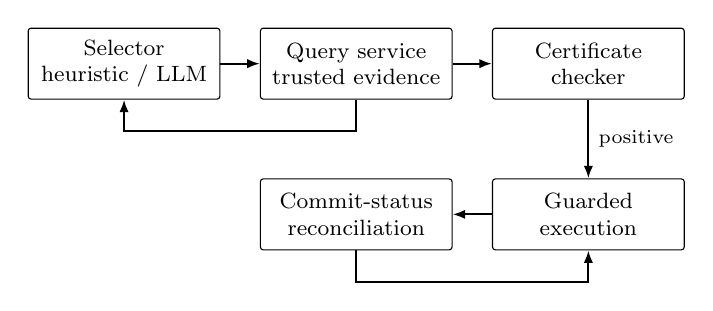
\begin{tikzpicture}[font=\footnotesize, node distance=7mm and 5mm,
 box/.style={draw,rounded corners=1pt,align=center,minimum height=9mm,text width=22mm},
 arr/.style={-{Latex[length=1.6mm]},thick}]
\node[box] (s) {Selector\\heuristic / LLM};
\node[box,right=of s] (q) {Query service\\trusted evidence};
\node[box,right=of q] (c) {Certificate\\checker};
\node[box,below=10mm of c] (e) {Guarded\\execution};
\node[box,left=of e] (r) {Commit-status\\reconciliation};
\draw[arr] (s)--(q);
\draw[arr] (q)--(c);
\draw[arr] (q.south) |- ([yshift=-4mm]s.south) -- (s.south);
\draw[arr] (c)--node[right,font=\scriptsize]{positive}(e);
\draw[arr] (e)--(r);
\draw[arr] (r.south) -- ++(0,-4mm) -| (e.south);
\end{tikzpicture}
\caption{The selector chooses evidence, not authority. Only a checked positive certificate permits a route to execute. Status evidence governs recovery after an ambiguous effect. Negative or unresolved decisions stop before actual execution.}
\label{fig:architecture}
\end{figure}

\subsection{Two types of query}
A \emph{run query} acquires a trusted receipt for one pair $(w,r)$. It records the bounded execution and whether $S(w,r)$ holds. This is a simulation of a declared candidate world. It does not reveal whether $w$ is the actual world. Repeating a query cannot create a new permission or turn a failed route into a successful one.

An \emph{initial-observation query} reads an allowed immutable initial value from the actual world. It can concern a file or a grant value. The possible answers of each public observation are defined over the catalog, but the actual answer is not available until acquisition. Observations reduce uncertainty about the world; they do not broaden authority. The distinction matters because learning that a write is needed is not the same as receiving permission to perform it.

Let $E$ denote the evidence acquired so far, and let $Q_E$ be its available observed queries with answers $a_q$. They define the compatible world set
\begin{equation}
 C(E)=\{w\in W:\ \forall q\in Q_E,\ q(w)=a_q\}.
 \label{eq:compatible}
\end{equation}
Unavailable observations remove no world. An answer inconsistent with the entire catalog produces a mismatch and abstention. The checker does not treat an empty compatible set as a vacuous proof that every world is safe. Acquisition runs in separate simulated states and does not consume the actual route's effect quota.

\subsection{Positive, negative, and unknown decisions}
A positive certificate identifies a single route that is supported in every compatible world. If $K_E$ is the table of paid run receipts, the condition is
\begin{equation}
 \exists r\in R\ \ \forall w\in C(E):\quad K_E(w,r)=\Yes.
 \label{eq:positive}
\end{equation}
Missing entries are unknown, not false. The certificate binds the program, world catalog, goal, grants, quota, semantics, and evidence references. A standalone checker reconstructs the compatible set and verifies receipt coverage without calling the interpreter. A public content hash identifies these inputs; it does not authenticate a fabricated receipt. Authenticity comes from the protected store assumed by the model.

A terminal negative needs two kinds of evidence. Every route must have an actual failure witness in the compatible set, and no permitted observation may still distinguish its relevant worlds. If a consumed observation was unavailable and could have separated the worlds, the result remains unknown. Exhausting a one-shot query list is therefore not enough to prove intrinsic impossibility. This rule prevents an availability failure from being relabelled as a property of the task.

An unknown outcome means that neither proof condition has been met. It can have different causes. A selector may have spent its budget on unhelpful queries. A useful observation may be unavailable. Alternatively, the true class may have no common successful route, but the selector has not acquired enough failure evidence to certify that fact. We retain these distinctions in the reference analysis. An unknown is not automatically a false block, and a negative is not automatically a failure to recognize a safe task.

\subsection{A small example}
Suppose two possible worlds contain different input formats. There are two format-specific routes and one robust route. Their success table is
\begin{equation}
\begin{array}{c|ccc}
 &r_A&r_B&r_C\\\hline
w_1&1&0&1\\
w_2&0&1&1
\end{array}.
\label{eq:example}
\end{equation}
Before any distinguishing observation, one successful receipt for $r_A$ in $w_1$ is insufficient. The actual world may be $w_2$. Two successful receipts for $r_C$ are sufficient, even though the actual world remains unknown. If a permitted format observation identifies $w_1$, one receipt for $r_A$ is sufficient after that observation. Evidence should resolve the execution decision, not necessarily identify every detail of the world.

Now remove $r_C$ and suppose no permitted observation distinguishes the two worlds. Each actual world has a successful route, but there is no single route that works for both. Increasing the query budget cannot create one. A controller that guesses may sometimes succeed, but that success is outside the robust certificate condition. This example explains the difference between actual-world feasibility and certifiable common-route feasibility.

\subsection{Soundness and the scope of stopping}
The contract assumes that the world catalog contains the actual world; the route set is closed; the interpreter, goal, grants, and quota are fixed; and the evidence is truthful and bound to the same initial snapshot. It also assumes that external state does not change before actual execution, acquisition does not mutate that state, and all effects pass through the gateway. These assumptions define the proof's scope. Later counterexamples show what breaks when they are removed.

\begin{proposition}[Positive soundness and preservation]
Under the stated assumptions, a route with a positive certificate completes the fault-free task in the actual world. The same route remains a valid witness after consistent additional evidence.
\end{proposition}
\emph{Proof.} Truthful filtering preserves $h\in C(E)$. The positive certificate contains a successful receipt for $(h,r)$, and the snapshot and semantics assumptions connect that execution to the actual one. After additional consistent evidence, the new compatible set is a nonempty subset of the old one. The old route still has a successful receipt for every remaining world.

This result supports stopping acquisition once the certificate exists. It does not say that later evidence leaves the checker's chosen route unchanged. The implementation chooses the first fully covered route. Later receipts may enable an earlier route in that ordering, even though the old witness remains valid. We therefore test witness success and full execution equality separately.

\begin{proposition}[Robust impossibility]
Let $B(h)$ contain all worlds with the same answers as $h$ to every permitted initial observation. If every route fails in at least one world in $B(h)$, no sound selector restricted to these queries can certify a common route, regardless of budget.
\end{proposition}
\emph{Proof.} No permitted observation removes a member of $B(h)$, and run queries reveal route outcomes without identifying the actual world. Every possible positive certificate would require one route to succeed throughout $B(h)$, contrary to the premise.

The proposition holds for each concrete transcript, including transcripts produced by randomized selectors. It does not prohibit success by a richer controller with new observations, new routes, or a different execution contract. Merely compressing a proof cannot create a common route that does not exist. The result also does not mean that each world individually lacks a successful route. The order of ``for every world'' and ``there exists a route'' is the key difference.

\subsection{A receipt-language lower bound}
At a fixed compatible set $C$, a positive certificate needs at least $|C|$ distinct successful run receipts for the same route. Each receipt covers only one world-route pair, so fewer receipts cannot cover the set. If a common route exists, acquiring its receipt in every world is sufficient. This is a bound on the explicit receipt language, not on all possible program analysis.

For unit-cost, always-available observations, a privileged hindsight minimum is
\begin{equation}
\begin{aligned}
L(h)=\min_{T\subseteq Q}\quad& |T|+|C_T(h)|\\
\text{subject to}\quad&\exists r\ \forall w\in C_T(h),\ S(w,r)=\Yes,
\end{aligned}
\label{eq:bound}
\end{equation}
where $C_T(h)$ is the class after obtaining observations $T$. The value is infinite if no such class admits a common route. An offline oracle can choose the useful observations and successful route with full knowledge. An actual selector cannot use that knowledge. We use $L(h)$ only to describe remaining acquisition overhead. A static analyzer or compressed proof could infer several outcomes without paying for separate receipts and would fall outside this bound.

\subsection{Selectors and online stopping}
All selectors use the same query catalog and certificate checker. Original-first acquires run queries in route/world order before observations. Route-cover favours routes with no observed failure, fewer missing compatible-world receipts, and lower public structural cost, with deterministic tie-breaking. Observe-cover first considers observations that split the compatible set, then uses the route-cover rule. If observation answers partition $C$ into groups of sizes $n_a$, its gain score is
\begin{equation}
\operatorname{gain}(q,C)=|C|-\frac{\sum_a n_a^2}{|C|}.
\end{equation}
Observe-cover takes the highest-scoring remaining observation when the gain is at least one. This score uses the public candidate partitions, not the actual answer or reference truth. The random control uses one fixed seed, so it is a reproducible control rather than an estimate over many random runs.

The LLM interface is intentionally small. The model chooses a valid query ID from the current public catalog. It does not supply free-form facts, a new policy, or a certificate. Source, source-plus-graph, and source-plus-padding views differ only in presentation. The graph contains deterministic data/control relations derived from all route programs. It adds no observation of the actual world. Padding controls the extra local input length without adding graph relations.

Algorithm~\ref{alg:acquire} describes online acquisition. The certificate check occurs before creating, reserving, or sending another model request. This order is essential for real call savings: detecting a certificate after dispatch would be too late to avoid that request. The fixed control follows the same acquisition interface but continues until its budget or catalog is exhausted. Its deliberate extra work measures the value of stopping within this contract.

\begin{algorithm}[t]
\caption{Evidence acquisition with certificate stopping}
\label{alg:acquire}
\begin{algorithmic}[1]
\Require Public case, query budget $b$, selector $\pi$
\State $E\gets\emptyset$
\For{$t=0,\ldots,b$}
  \State $d\gets\operatorname{Check}(E)$
  \If{$d$ is observation mismatch}
    \State \Return mismatch / abstention
  \EndIf
  \If{$d$ is positive or terminal negative}
    \State Verify $d$ against the trusted store; \Return $d$
  \EndIf
  \If{$t=b$ or no query remains}
    \State \Return unknown
  \EndIf
  \State $q\gets\pi(\text{public case},E,\text{remaining IDs})$
  \If{selection or provider response is invalid}
    \State \Return decision supported by the valid paid prefix
  \EndIf
  \State Acquire trusted answer to $q$; append it to $E$
\EndFor
\end{algorithmic}
\end{algorithm}

\subsection{Recovery after an ambiguous effect}
Recovery begins only after the caller has verified the route certificate. The executor keeps the same route, allows at most four attempts, and shares the quota between effects and status requests. It restarts that route using exact cached receipts, including the original read values. This avoids reading a value changed by an earlier write during the retry. It does not combine a safe prefix from one route with an uncertified suffix from another.

We compare three policies. Strict-stop abstains after an ambiguous result. Terminal-status uses a bounded status request. A confirmed committed record supplies the original receipt and permits continuation. A terminal-noncommit record permits a fresh generation only if it also fences the old attempt, meaning the old request can no longer commit. Pending, absent, unavailable, stale, or mismatched records do not permit continuation. This rule separates ``no result was found'' from ``the effect definitely did not and cannot occur''.

Same-ID deduplication is a separate control. It relies on a backend that atomically stores operation identities and their outcomes. That is a stronger backend capability, not merely another interpretation of the same information. In this implementation, a fixed ID that has reached terminal noncommit remains terminal; replaying it does not create a successful new generation. The comparison therefore evaluates different recovery contracts, not universal dominance of one retry strategy.

Operation identity binds the run epoch, route, logical effect key, and attempt generation. Status binds that identity to the operation, resource, value, and grant context. Every dispatched effect, including a denied or deduplicated call, consumes quota. Exact local receipt reuse is free. A status query consumes both shared quota and its separate status budget. Even valid recovery can therefore exhaust resources needed by the suffix; authorization and duplicate prevention do not guarantee liveness.

The recovery invariant is simple: the controller must not dispatch a second live attempt for a logical effect merely because the first reply is missing. A committed record allows reuse of the result; a fenced noncommit allows a new attempt; unresolved status allows neither. The implementation assumes trustworthy, durable status and receipt binding. It is not a verified implementation of distributed storage, network authentication, or garbage collection.

\section{Implementation and Experimental Design}
\label{sec:design}
\subsection{Prospective freezes and synthetic data}
The latest research release is Phase 11. Its production sources and analysis plan were locally hash-frozen before heldout materialization and model acquisition. Data were then frozen before the API outcomes were observed. These records provide a checkable chronology, but they are local prospective records, not an external preregistration. The paper is a new reporting artifact; it does not alter the frozen release.

The main cohort contains 48 cases from 24 structural families, with two lexical variants per family. A separately tasked AI coding agent generated the cases without reading the new production implementation or model outcomes. The reference uses a separate implementation of the guarded semantics. This separation reduces shared-code bias, but it is not independence from the written specification, prior infrastructure, or the overall research process. It is not independent human annotation.

An aggregate coverage check found an important weakness in the main cohort: every feasible fully observed class was a singleton. Such cases can show that observations help identify a world, but provide limited evidence that a common route can be certified while several worlds remain possible. Before API outcomes, we added a separate challenge cohort of 24 cases from 12 families. Nine families support multiworld positive certificates; three have no common route even though each world has a route; two permit no observation savings. These categories overlap. We preserve the original cohort and report both cohorts separately.

Twelve further cases vary the numbers of worlds and routes in one shared scaling construction. They are dependent siblings, not twelve new independent families. Table~\ref{tab:data} gives the main denominators. The 218 actual-world rows expand cases over possible actual worlds. Repeating those rows over budgets, faults, and policies produces experimental conditions, not additional independent tasks.

\begin{table}[t]
\centering
\caption{Dataset structure. Scaling is reported separately.}
\label{tab:data}
\begin{tabular}{lrrr}
\toprule
Cohort & Families & Cases & Actual-world rows\\
\midrule
Main &24&48&102\\
Challenge &12&24&116\\
Combined &36&72&218\\
Scaling siblings &1 construction&12&90\\
\bottomrule
\end{tabular}
\end{table}

\subsection{Executable truth and independent checks}
The reference checks every world-route pair, including the scaling cases, for 1,006 comparisons. It compares final files, emissions, success, defined errors, and execution accounting. Two raw error strings differ only because one includes the unbound variable's name. The original disagreements remain in the archive. A separately documented typed-error normalization yields agreement on all 1,006 pairs. Reporting both counts avoids presenting a later normalization as an initially perfect match.

Small evidence states receive additional checks. The main reference exhaustively tests 8,672 cache/history states. The challenge reference tests 371,072 states across its tractable partitions, plus 180 boundary checks for six broader partitions. The latter are not called exhaustive. Separate theorem tests enumerate small Boolean success tables and compatible refinements. These tests support the implementation and expose edge cases; they do not replace the mathematical arguments or establish correctness for arbitrary programs.

We also retain explicit assumption counterexamples. They cover an omitted actual world, state drift after certification, forged replacement of the trusted store, and an absence-based unsafe retry. These cases are not counted as normal benchmark failures because they deliberately violate a premise or use an unsafe controller. Their purpose is to make each guarantee's boundary executable and inspectable.

\subsection{Deterministic and recovery grids}
The acquisition grid crosses all declared actual worlds with four selectors, budgets 2, 4, 8, 12, and full, and stopping on/off. Full means the public query catalog size for that case. This gives 12,320 conditions, including the separate scaling stratum. Every returned certificate is checked against the trusted cache. Every positive certificate is followed by actual fault-free route execution within the synthetic environment.

The recovery grid contains 15,696 conditions. It combines all main/challenge actual-world rows with twelve fault schedules, three recovery policies, and status budgets zero or one. The faults include no fault, a commit with a lost acknowledgement, terminal noncommit, pending status, unavailable status, stale status, wrong signature, and absence while pending. Additional schedules place terminal faults at a later mutation or an emit. The primary comparisons use the first-mutation terminal faults with one status request available.

Missing certificates and untriggered fault targets remain in the unconditional denominators. We also report the triggered, certifiable subset where appropriate. This distinction prevents a recovery rate from hiding tasks that never reached the fault. The controller cannot claim recovery simply because an injected event was never encountered.

\subsection{Live model acquisition and integrated execution}
The live experiment uses GPT-6 Luna and GPT-4.1 mini, recorded by the model identifiers returned in the campaign artifacts. For each of 36 families, it selects the first lexical variant and one actual world using a deterministic hash rule. Each model runs in four cells: source online, graph online, padding online, and source fixed. The total is $36\times2\times4=288$ streams. These fresh cells use separate request identities; one cell does not reuse another cell's model decisions.

Each stream allows at most twelve query selections and 1,024 output tokens per request. There are no automatic retries or fallback models. The parser accepts a unique valid final selection under the declared response schema. Provider errors remain recorded failures. A valid prefix can still support a certificate, so full-stream validity and prefix-supported completion are separate measurements. No missing model choice is reconstructed during offline replay.

Graph and padding inputs have equal token counts under the local \code{o200k\_base} encoding. This is a reproducible length control, not proof that the provider uses that tokenizer for GPT-6 Luna. We record provider usage separately and avoid claiming exact provider-token matching. The comparison asks whether graph relations offer an advantage beyond the locally matched extra input, within the tested prompts and models.

Every acquired stream prefix is replayed at budgets 2, 4, 8, and 12, under four fault settings and three recovery policies. This produces 13,824 integrated conditions. The same checker and executor are used after model acquisition, so a better-looking query sequence counts as useful only if it yields a certificate and supports task completion. A separate matched-prefix analysis compares the earliest positive witness with a later witness from the same recorded stream.

\subsection{Measures and statistical treatment}
The primary completion endpoint requires error-free authorized termination and a satisfied goal. We call it \emph{acknowledged completion}. Physical goal satisfaction checks only whether the final files and emissions meet the goal. These endpoints can differ after a lost acknowledgement: the write may already exist although the controller cannot confirm completion. Physical-goal recovery results were added after outcome review and are labelled posthoc throughout.

For deterministic conditions, we first average the relevant worlds and lexical variants within each structural family. We then weight the 36 families equally. If $y_{fi}$ is an outcome for row $i$ of family $f$, the reported mean is
\begin{equation}
\bar y=\frac{1}{F}\sum_{f=1}^{F}\left(\frac{1}{n_f}\sum_{i=1}^{n_f}y_{fi}\right).
\end{equation}
This differs from dividing all successful rows by all rows when families have different sizes. Model comparisons use one actual world per family, so their 36-task denominator must not be confused with the 218-row deterministic denominator.

Comparisons use paired family effects. We resample those effects 10,000 times with seed 11101 and report the 2.5th and 97.5th percentiles. The resulting 95\% intervals are descriptive summaries over authored templates. They are not population confidence guarantees, and we report no significance tests or claims of generalization to deployed Skills. The one model draw per cell also means that these intervals do not measure model run-to-run variability.

Work is a vector rather than a single score: acquired queries, interpreter calls and steps, initial reads, checker comparisons, actual effects/status requests, provider tokens, estimated cost, and request elapsed-time sums. Selector partition scoring, parsing, standalone-checker CPU, and operating-system overhead are excluded from the abstract operation counters. A reduction in those counters is therefore not a measured total-CPU or wall-clock speedup. Dollar values are conservative rate-based estimates with reserved exposure for unknown usage, not provider invoices.

\subsection{Isolation and replay}
The experiment executes only the synthetic language. Restricted Docker runs use no network or host mounts, a read-only root filesystem, UID 65534, dropped capabilities, no new privileges, and bounded CPU, memory, process count, and temporary storage. There are 117 deterministic and 56 integrated batches, with fresh semantic state for each condition. The pinned image identifier and batch records are retained. A fresh container rerun requires that image locally.

Reproducibility has two meanings here. Deterministic replay reconstructs cases, evidence, certificates, executions, and analyses from archived records. It does not require a model API key. Fresh API acquisition would make new stochastic requests and is not expected to reproduce the same answers. Similarly, checking recorded container evidence is not a new container launch. The artifact documentation keeps these procedures separate so that a successful replay is not mistaken for a new independent experiment.

The reproduction environment uses Python 3.12, locked dependencies, and a checked tokenizer cache. After setup, \code{scripts/hydrate\_phase11.py} restores archived working inputs. Running \code{scripts/verify\_phase11.py} then checks hashes and recomputes the recorded evidence with network calls blocked. The accompanying reproduction guide specifies dependency setup and a separate procedure for fresh container runs.

\section{Results}
\label{sec:results}
\subsection{Stopping reduces work while preserving completion}
At budget twelve, observe-cover uses a mean of 7.750 queries under fixed acquisition and 3.014 with certificate stopping. The paired difference is $-4.736$ queries, with a descriptive interval of $[-5.556,-3.944]$. Family-mean completion is 81.94\% in both conditions. The corresponding raw count is 178 successful actual-world rows out of 218; its raw percentage is not the family mean.

The savings also appear in other measured work. Mean interpreter steps fall from 29.000 to 6.111, while certificate pair checks fall from 69.111 to 50.611. Mean interpreter calls fall from 6.722 to 2.097. These results support RQ1 within the measured interface: once the checker has enough evidence, further acquisition often adds cost without enabling more completion. They do not show that checking itself is free or that the selector is globally optimal.

\begin{figure*}[t]
\centering
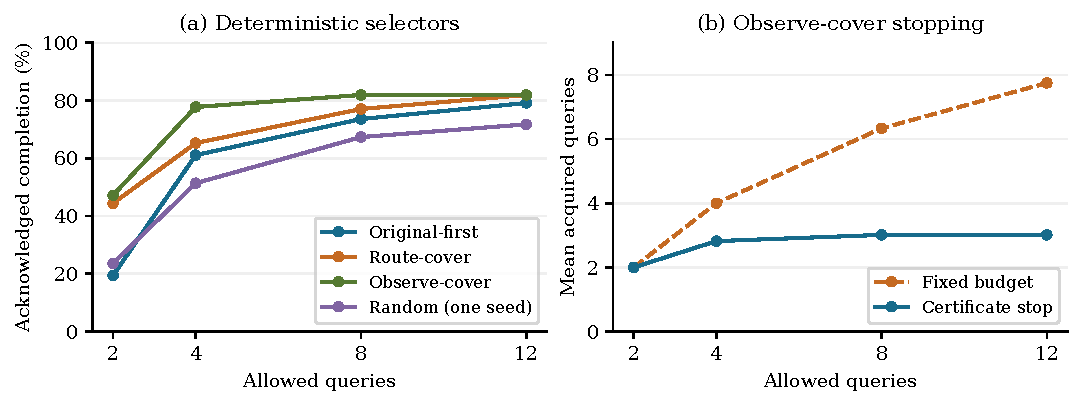
\includegraphics[width=.96\textwidth]{acquisition.pdf}
\caption{Acquisition on the 36-family combined cohort. (a) Completion under online stopping for four deterministic selectors. (b) Observe-cover's acquired work with and without certificate stopping. Points are equal-family means over dependent worlds and variants; scaling siblings are excluded. The random curve uses one fixed seed.}
\label{fig:acquisition}
\end{figure*}

At full budget, the mean query difference is $-6.153$ with interval $[-8.139,-4.514]$, again with unchanged completion. At budget twelve, main-family completion is 85.42\% and challenge-family completion is 75.00\%. Observe-cover already reaches this ceiling at budget eight and leaves no unresolved unknowns: the remaining forty actual-world rows have negative certificates. A lower completion ceiling is therefore not necessarily caused by poor acquisition. Some cases cannot meet the fixed-route condition.

Figure~\ref{fig:acquisition} shows why the comparator matters. Acquisition policies differ at small budgets, even though they share the same checker. A weak ordering can spend its budget proving unhelpful routes. Observe-cover uses public structure to choose useful observations and missing receipts. It is a strong control within this catalog, rather than a deliberately uninformed baseline. However, the experiment does not compare it with the established decision-region algorithms discussed in Section~\ref{sec:related}.

The hindsight bound gives another limited perspective on efficiency. Among positive families at full budget, observe-cover's mean gap from the privileged minimum is 0.2 queries. This gap is conditional on a positive certificate and excludes the forty infeasible world rows. It suggests little remaining acquisition headroom on these feasible templates under this receipt language. It does not establish optimal expected behaviour without hindsight, or efficiency under a different proof interface.

\subsection{Models do not improve the matched end-to-end result}
The matched model comparison uses one actual world from each family. At budget twelve, observe-cover completes 30 of the 36 selected tasks. GPT-6 Luna completes 29 and GPT-4.1 mini completes 28. Their mean query counts are 4.583 and 5.639, compared with 3.000 for observe-cover. Table~\ref{tab:model} and Figure~\ref{fig:models} show the result and its cohort structure.

\begin{table}[t]
\centering
\caption{Source-online comparison at budget twelve. Each family contributes one selected actual world.}
\label{tab:model}
\begin{tabular}{lrrrr}
\toprule
Selector & Main & Challenge & Total & Queries\\
\midrule
Observe-cover &21/24&9/12&30/36&3.000\\
GPT-6 Luna &21/24&8/12&29/36&4.583\\
GPT-4.1 mini &21/24&7/12&28/36&5.639\\
\bottomrule
\end{tabular}
\end{table}

Relative to observe-cover, the completion difference is $-2.78$ percentage points for Luna, with interval $[-8.33,0]$, and $-5.56$ points for mini, with interval $[-13.89,0]$. The query differences are $+1.583$ $[1.000,2.222]$ and $+2.639$ $[1.944,3.361]$. These finite comparisons do not prove that models are always worse. They do show that this experiment provides no evidence of a model advantage over the capable heuristic.

The challenge cohort is especially informative. All three selectors complete 21 of 24 main tasks, so the main cohort alone gives little separation in completion. On the challenge cases, the heuristic completes nine, Luna eight, and mini seven. The added structures expose acquisition failures that would have been hidden by relying only on the main cohort. Because the challenge was commissioned after a coverage review, we report it as a separate designed stress test rather than an untouched random holdout.

\begin{figure*}[t]
\centering
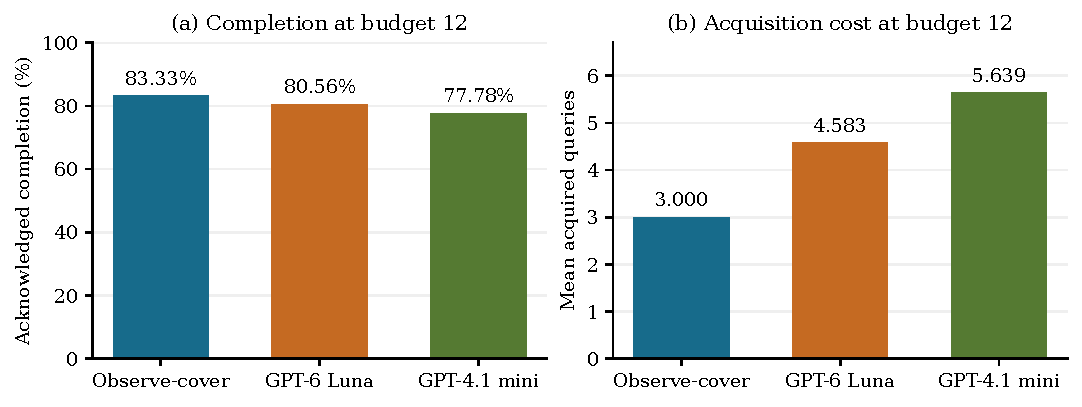
\includegraphics[width=.96\textwidth]{models.pdf}
\caption{Matched source-online results on 36 selected actual worlds at budget twelve. The same evidence checker and executor follow each selector. Model-selected queries do not yield higher completion and require more acquisitions than observe-cover. These are single provider draws per cell, not estimates over repeated model runs.}
\label{fig:models}
\end{figure*}

The result also explains why an apparent query-level improvement may fail to become an end-to-end gain. A certificate needs complete support for one route, not merely several useful-looking receipts. Extra queries on different routes can leave each route partly covered. Once a strong heuristic already reaches the feasible ceiling, changing the order of redundant queries cannot increase completion. In this study, the measured outcome is the certificate and executed goal; we do not infer hidden reasoning quality from the model's query text.

\subsection{Unknowns have more than one cause}
Across all 288 streams, 230 finish with a positive certificate, 43 with a negative certificate, and 15 remain unknown. The independent reference identifies ten of the unknown streams as still certifiable. These are acquisition failures under the available interface and budget: enough evidence could have supported a common route, but the stream did not obtain it. The other five unknowns occur in robustly infeasible classes whose negative proof was not completed.

This distinction changes the interpretation of unknown rates. More effective query ordering could help the ten certifiable streams. It could help the other five produce a clearer negative answer, but it could not create a common route. Allowing execution in those cases would require a different contract, such as an extra permitted observation or an additional route. Simply increasing the model's confidence would not repair the missing logical condition.

Protocol reliability is a separate axis. There are 1,605 provider responses, of which 1,603 yield valid selections, and 286 fully valid streams. Two Luna requests return HTTP 400 with an invalid-prompt error category. The retained records do not include enough error-message detail to assign a more specific cause. We therefore do not describe these errors as confirmed safety refusals or infer a particular provider restriction. All failed streams remain in the denominators.

The archive contains no budget rejection and no uncertain transport event for this campaign. The fifteen unknowns should therefore not be described as requests stopped by the spending cap. Their task-level interpretation comes from the reference outcome, while provider validity is reported separately. A small protocol error rate and a small unknown rate are useful diagnostics, but neither alone establishes successful task completion.

\subsection{Graph effects do not survive a stronger control}
At budget twelve, graph minus source completion is $+1/36$ for Luna and zero for mini. Against padding, the completion difference is zero for both models. Graph minus padding query differences are $-0.278$ $[-1.000,0.361]$ for Luna and $+0.139$ $[-0.250,0.694]$ for mini. The direction is not consistent across the two models.

The source-only comparison might suggest a graph benefit for Luna. The padding comparison weakens that interpretation because it adds a similar amount of input without adding graph relations. The observed change could reflect altered attention, input length, or query ordering. The evidence does not isolate a stable benefit from graph edges themselves. This is a useful negative result for RQ3, rather than a claim that graphs can never help.

The design also limits the opportunity for a graph to add value. The source already contains all the information used to construct the graph. The cases are small and their route catalogs are closed. A strong deterministic selector can inspect public partitions and receipt coverage directly. A graph may become more useful on larger programs or when it exposes relations absent from the baseline view, but that would require a separate information-controlled experiment.

\subsection{Fresh online stopping reduces acquired API cost}
Fresh source-online streams use fewer queries than separately acquired source-fixed streams. Luna's mean falls from 7.639 to 4.583, and mini's from 7.750 to 5.639. Aggregate completion remains equal within each model. This does not imply per-family equivalence: Luna has one family win and one loss between the fresh cells. Independent model draws can change the path before a certificate is reached.

Table~\ref{tab:cost} reports conservative per-stream cost estimates. Luna saves USD 0.003521 per stream, with interval [0.002293, 0.004882]. Mini saves USD 0.008588, with interval [0.004519, 0.013407]. These savings concern acquired requests under the recorded rates and usage. They differ from an offline calculation of requests that could have been avoided after the campaign.

\begin{table}[t]
\centering
\caption{Fresh source-stream acquisition. Costs are conservative mean estimates in USD, not invoices.}
\label{tab:cost}
\begin{tabular}{llrr}
\toprule
Model & Mode & Queries & Cost / stream\\
\midrule
Luna &Fixed&7.639&0.008276\\
Luna &Online&4.583&0.004755\\
mini &Fixed&7.750&0.027075\\
mini &Online&5.639&0.018487\\
\bottomrule
\end{tabular}
\end{table}

The matched-prefix analysis addresses a different question: does an earlier positive witness remain valid when more evidence is present? All 670 matched positive comparisons succeed with both the first and later witness. Only 621 have identical full execution results. The other cases remain successful but can choose a different route or trace. This directly supports the preservation statement while rejecting the stronger claim of full trajectory equality.

The entire Phase 11 acquisition uses 13,502,244 known input tokens and 23,056 known output tokens. Its conservative additional cost is \$3.76518, including retained reservations for two responses with unknown usage. Cost is reported for transparency, not as an economic claim about future model prices. The paper-writing stage makes no additional experimental API calls.

\subsection{Recovery resolves knowledge and sometimes adds progress}
With one status request, terminal-status reaches acknowledged completion in 178 of 218 world rows under each primary terminal fault. Strict-stop reaches acknowledged completion in zero rows in these conditions. The equal-family gain is 81.94 percentage points, with interval $[69.44,93.06]$. Conditional on a certificate and a triggered fault, terminal-status recovers all 178 of 178 executions. This conditional ceiling follows the usable-status contract and should not be presented as tolerance of arbitrary network failures.

The physical-goal analysis gives a more precise account of the gain. When the first mutation commits but its acknowledgement is lost, strict-stop already satisfies the physical goal in 84 of 218 rows, or 38.89\% as a family mean. Terminal-status reaches 178 rows and 81.94\%. The physical-goal gain is therefore 43.06 points, with interval $[27.78,59.72]$, rather than the 81.94-point gain in acknowledged completion. Figure~\ref{fig:recovery} keeps both endpoints visible.

\begin{figure*}[t]
\centering
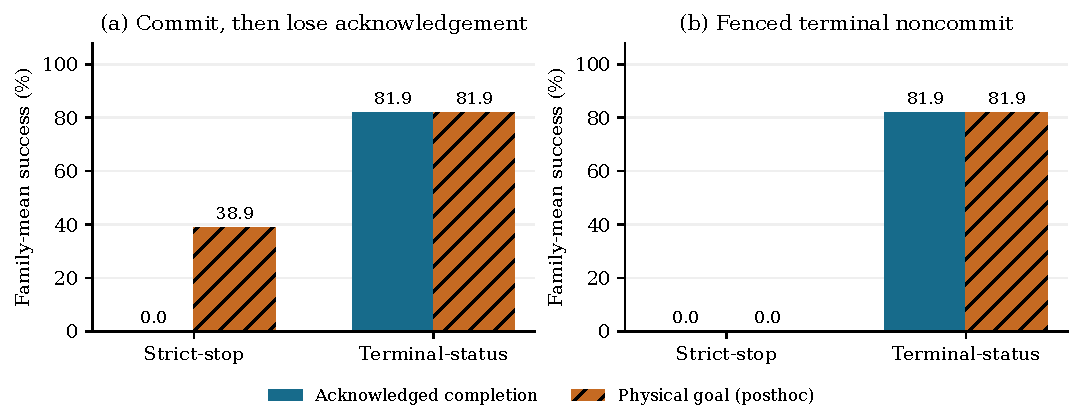
\includegraphics[width=.96\textwidth]{recovery.pdf}
\caption{Recovery on all 218 main/challenge actual-world rows with one status request available. The y-axis uses equal-family means. A lost acknowledgement can leave the physical goal already satisfied, so acknowledged recovery and new task progress are different. Physical-goal analysis is a separately retained posthoc addition.}
\label{fig:recovery}
\end{figure*}

Under terminal noncommit, strict-stop has no corresponding physical progress, so the acknowledged and physical-goal gains coincide. In the committed-but-unacknowledged case, recovery combines two benefits: confirming an effect that already happened and allowing any remaining suffix to run. The primary endpoint measures both. The posthoc endpoint isolates physical state more clearly, but it does not retroactively become a prespecified primary outcome.

Recovery remains appropriately limited when the status is unresolved. Pending, absent-while-pending, unavailable, stale, and wrong-signature status do not complete these first-mutation cases under terminal-status. Same-ID deduplication handles the committed ambiguity, but does not complete terminal-noncommit cases in this implementation because the fixed operation ID remains terminal. These findings support RQ4's distinction between evidence types, not a general ranking of all recovery systems.

The absence counterexample explains why this restriction is necessary. An unsafe controller sees no record, sends a fresh-ID retry, and then allows the delayed original to commit. The trace contains a duplicate logical effect. The terminal-status and same-ID controls abstain in that pending schedule. Absence can be fresh and still be insufficient; what matters is whether the old attempt is prevented from committing.

\subsection{Trace checks, scaling, and the previous version}
All 43,064 recorded restricted-container conditions agree exactly with local replay. This total includes 8,664 top-level null results, and some policy wrapper records contain an additional null execution field. It is therefore not a count of 43,064 successful or even attempted executions. The separate trace audit reports the execution denominator explicitly.

That posthoc audit covers 42,846 slots across semantic, policy, recovery, and integrated records, excluding the 218 previous-contract comparisons. It contains 28,482 actual executions and 14,364 nulls. The auditor checks 63,622 recorded commits, including 50,608 mutations, and finds zero unauthorized commits and zero duplicate logical mutations. Forty unauthorized dispatch attempts in negative semantic routes are denied. The audit reconstructs final states and quota charges without trusting the runtime's summary counter.

These zero counts require careful interpretation. The runtime's own unauthorized-effect field is fixed to zero by the guarded construction, so it is not an independent security measurement. The separate auditor improves the check by examining recorded signatures and logical identities. It still assumes complete and truthful simulator traces. Neither count establishes a real-world prompt-injection attack rate or resistance to compromise of the trusted process.

The scaling siblings expose a cost of explicit receipts. In the full fixed grid, acquired run queries range from four for two worlds and two routes to 128 for sixteen worlds and eight routes. These counts reflect the deliberately expanded world-route table. They do not demonstrate general asymptotic performance for arbitrary programs. A richer proof language could compress equivalent executions; the present lower bound would then no longer apply unchanged.

The previous Phase 10 controller and the new full-budget contract complete the same 178 of 218 actual-world rows. The comparison uses different acquisition and planning interfaces, so it cannot isolate the causal effect of one repair. The supported improvement is clearer evidence accounting and reduced acquisition after sufficient evidence, not a new full-information completion ceiling. Earlier results remain archived rather than being recalculated under the new definitions.

\section{Discussion and Limits}
\label{sec:discussion}
\subsection{What the results establish}
The strongest finding is that useful stopping depends on the decision being certified. A detector-style label over the whole input is not required to prove that one fixed route can complete the goal. Conversely, knowing that each world has some successful route is not enough when the controller must choose one route before the worlds can be distinguished. The positive and negative certificate conditions make these differences explicit.

The study also separates acquisition quality from authority. A model can choose an inefficient query without gaining permission to execute an unsupported route. The checker absorbs that uncertainty by withholding a certificate. This separation makes the negative model results meaningful: poor query efficiency affects cost and completion, but is not silently converted into a broader permission. It also explains why a more expressive model is not automatically a better controller for a small, fully structured query catalog.

There is a corresponding lesson for recovery. A stronger tendency to retry is not the same as better availability. Legal recovery depends on the state of the prior operation and the backend's guarantees. Terminal evidence can safely recover useful work; an unresolved operation can make abstention the correct outcome. Evaluations should therefore report fault types and evidence availability, rather than one undifferentiated recovery percentage.

\subsection{Internal validity and measurement limits}
Several choices strengthen the internal checks: a separate reference, prospective local freezes, retained errors, paired family comparisons, and recorded end-to-end execution. They do not remove all shared assumptions. The generator and implementation share a written contract and some prior diagnostic infrastructure. Agreement can validate a common interpretation while missing a weakness in the interpretation itself. The counterexamples help expose this boundary but cannot enumerate every omitted assumption.

The dataset is authored and small. Two lexical variants test superficial changes, not broad semantic diversity. The challenge supplement was added after a known coverage gap, and the scaling cases share one construction. A single random seed and one API draw per model/cell leave stochastic robustness unresolved. The intervals summarize variation over these families only. More repeated requests on the same templates would not, by themselves, establish wider structural generalization.

The work measures are incomplete by design. Observe-cover's partition scoring and structural analysis have costs that are excluded from the operation vector. We therefore cannot conclude that fewer purchased queries imply lower total computing cost in every setting. A fair deployment study would measure full wall time, CPU, memory, and any cost of generating the candidate worlds. It would also compare against a competitive static analyzer and established decision-region acquisition methods.

Protocol changes across phases create another limit. A posthoc audit of 1,587 older decisions accepts thirteen previously rejected responses with explicit commentary and a unique final answer, without rejecting an older valid decision. This diagnoses an extraction problem. It does not reconstruct the missing later decisions of those adaptive streams, and it does not justify rewriting old completion rates. The fresh campaign changes several details together, so its reliability cannot be attributed solely to a simpler protocol.

\subsection{External validity and security scope}
The finite world catalog is the central restriction. Real systems may contain unknown files, changing dependencies, hidden service state, or behaviours that the language cannot express. If the actual state is absent from the catalog, a complete certificate over the listed worlds can still be wrong for reality. If state changes after certification, the same problem arises over time. Neither more model confidence nor a content hash repairs these violations.

The trusted store, gateway, and status backend are also substantive assumptions. A selector that can replace the cache may construct internally consistent hashes for false records. The forged-store counterexample makes that failure visible. Recovery assumes authenticated binding, durable records, retention, atomicity, and fencing. We model those properties rather than implement and verify a distributed service that provides them.

For these reasons, the paper supports a systems mechanism study, not a general Skill security product. It contains no new real-Skill evaluation, malicious-Skill prevalence estimate, or human-labelled test set. Its relevance to agent security lies in a precise interface between uncertain selection and constrained execution. Transferring the mechanism to open-ended agents would require a new account of state coverage, policy correctness, and complete interception of effects.

\section{Conclusion and Future Work}
\label{sec:conclusion}
This study asked when an agent has enough evidence to execute a bounded workflow and when it can continue after an ambiguous effect. The proposed contract separates three questions: whether an action is authorized, whether one route completes the goal in all compatible worlds, and whether a prior effect has committed. A query selector gathers evidence, a separate checker validates it, and a recovery controller uses typed status records. The separation makes both success and abstention easier to explain.

The experiment answers RQ1 with a clear but scoped result. Certificate stopping reduces observe-cover's mean acquired queries from 7.750 to 3.014 at budget twelve, while preserving 81.94\% family-mean completion. The matched-prefix checks support preservation of a successful witness, not preservation of the entire trace. This is evidence that the explicit stopping condition avoids unnecessary acquisition within the contract. It is not a new optimal stopping theorem or a complete account of system cost.

RQ2 shows why unknown outcomes should be classified before they are optimized. Ten of the fifteen unknown model streams remain certifiable under the reference, while five have no robust common route but lack a completed negative proof. Better acquisition can help the first group complete and the second group explain its limitation. It cannot remove the difference between an actual-world route and a route that works across an indistinguishable class. This is the main conceptual value of the negative certificate.

RQ3 yields a negative comparative finding. The two models complete fewer matched tasks and use more queries than observe-cover. Graph augmentation does not show a stable advantage over locally token-matched padding. These outcomes suggest that public structure and a focused deterministic policy are strong competitors in small query spaces. Future work should retain such controls instead of using only weak query orders. It should also test repeated model draws and report the cost of the heuristic's own computation.

RQ4 confirms that recovery needs stronger evidence than missing output. Committed receipts and fenced terminal noncommits support continuation in the modeled terminal cases. Pending or absent status does not. The physical-goal analysis further shows that acknowledged recovery can partly confirm work already done. A future recovery benchmark should prespecify both endpoints and vary record retention, fencing failure, stale reads, concurrent writers, and faults in the status service itself.

The next methodological step is to improve the evidence interface rather than simply enlarge the model. A useful extension would compare explicit receipts with a sound static analyzer or a compressed certificate that covers equivalent worlds. Another would implement established decision-region selectors with the same information and cost accounting. These comparisons could reveal whether the present acquisition savings come from the contract, the selector, or the representation of proof. They would also test how much of the receipt-language lower bound is avoidable through better reasoning tools.

Broader validation should preserve the current study's separation of assumptions and outcomes. New synthetic generators should introduce different control structures, noisy or unavailable observations, and controlled state changes before model results are inspected. Repeated trials should be grouped by structural family, with enough independent structures to support a meaningful generalization question. Fresh data should remain separate from development and challenge sets. The aim should be to find where the contract fails, not to choose cases that make a preferred method win.

The reproducibility package provides a starting point for that work. It retains old results, frozen inputs, raw model responses, reference checks, counterexamples, container records, per-family tables, and figure sources. Deterministic replay can verify the recorded claims without new API spending. Future hosted-model outputs may change, so historical replay and new acquisition must remain separate. The resulting contribution is a transparent, testable account of sufficient evidence and legal recovery in a bounded setting, with clear limits on what it says about real agents.

\section*{Author Contributions}
\balance
Victor Cao and Enlin Li report equal overall contributions (50\% each) to the project and this report. In the initial literature review, Victor led the review of threats and benchmarks, and Enlin led the review of defence methods.

\section*{Artifact Availability}
The source, raw evidence, and reproduction instructions are retained in the accompanying \href{https://github.com/victorcao1104/taskskillguard-research}{private research repository}. This report uses research release \code{088af27} and the append-only CI portability amendment \code{b994ef8}. The artifact guide identifies the full commit hashes and commands. Repository access must be provided to reviewers; no public artifact release is claimed.

\clearpage
\nobalance
\IEEEtriggeratref{11}
\begin{thebibliography}{20}
\bibitem{liu} Y. Liu \emph{et al.}, ``Do not mention this to the user: Detecting and understanding malicious Agent Skills in the wild,'' in \emph{Proc. USENIX Security Symp.}, 2026, pp. 1727--1746. [Online]. Available: \url{https://www.usenix.org/conference/usenixsecurity26/presentation/liu-yi}
\bibitem{skillinject} D. Schmotz, L. Beurer-Kellner, S. Abdelnabi, and M. Andriushchenko, ``Skill-Inject: Measuring agent vulnerability to Skill file attacks,'' \emph{arXiv:2602.20156v3}, 2026, doi: \href{https://doi.org/10.48550/arXiv.2602.20156}{10.48550/arXiv.2602.20156}.
\bibitem{injecagent} Q. Zhan, Z. Liang, Z. Ying, and D. Kang, ``InjecAgent: Benchmarking indirect prompt injections in tool-integrated large language model agents,'' in \emph{Findings of ACL}, 2024, pp. 10471--10506, doi: \href{https://doi.org/10.18653/v1/2024.findings-acl.624}{10.18653/v1/2024.findings-acl.624}.
\bibitem{context} F. Holzbauer, D. Schmidt, G. Gegenhuber, S. Schrittwieser, and J. Ullrich, ``Context matters: Repository-aware security analysis of the Agent Skill ecosystem,'' \emph{arXiv:2603.16572v2}, 2026, doi: \href{https://doi.org/10.48550/arXiv.2603.16572}{10.48550/arXiv.2603.16572}.
\bibitem{skillmutator} Y. Kim, M. Song, and S. Shin, ``SkillMutator: Benchmarking and defending language-and-code cross-modal attacks on LLM Agent Skills,'' \emph{arXiv:2606.14154}, 2026, doi: \href{https://doi.org/10.48550/arXiv.2606.14154}{10.48550/arXiv.2606.14154}.
\bibitem{agentdojo} E. Debenedetti, J. Zhang, M. Balunovic, L. Beurer-Kellner, M. Fischer, and F. Tram\`er, ``AgentDojo: A dynamic environment to evaluate prompt injection attacks and defenses for LLM agents,'' in \emph{Advances in Neural Information Processing Systems}, vol. 37, 2024, doi: \href{https://doi.org/10.52202/079017-2636}{10.52202/079017-2636}.
\bibitem{asb} H. Zhang \emph{et al.}, ``Agent Security Bench (ASB): Formalizing and benchmarking attacks and defenses in LLM-based agents,'' in \emph{Proc. Int. Conf. Learning Representations}, 2025. [Online]. Available: \url{https://openreview.net/forum?id=V4y0CpX4hK}
\bibitem{struq} S. Chen, J. Piet, C. Sitawarin, and D. Wagner, ``StruQ: Defending against prompt injection with structured queries,'' in \emph{Proc. USENIX Security Symp.}, 2025, pp. 2383--2400. [Online]. Available: \url{https://www.usenix.org/conference/usenixsecurity25/presentation/chen-sizhe}
\bibitem{ipiguard} H. An \emph{et al.}, ``IPIGuard: A novel tool dependency graph-based defense against indirect prompt injection in LLM agents,'' in \emph{Proc. EMNLP}, 2025, pp. 1023--1039, doi: \href{https://doi.org/10.18653/v1/2025.emnlp-main.53}{10.18653/v1/2025.emnlp-main.53}.
\bibitem{drift} H. Li, X. Liu, H.-C. Chiu, D. Li, N. Zhang, and C. Xiao, ``DRIFT: Dynamic rule-based defense with injection isolation for securing LLM agents,'' in \emph{Advances in Neural Information Processing Systems}, vol. 38, 2025, doi: \href{https://doi.org/10.52202/085713-2791}{10.52202/085713-2791}.
\bibitem{skillscope} J. Wu \emph{et al.}, ``SkillScope: Toward fine-grained least-privilege enforcement for Agent Skills,'' \emph{arXiv:2605.05868v3}, Sep. 2026, doi: \href{https://doi.org/10.48550/arXiv.2605.05868}{10.48550/arXiv.2605.05868}.
\bibitem{progent} T. Shi \emph{et al.}, ``Progent: Securing AI agents with privilege control,'' \emph{arXiv:2504.11703v3}, May 2026, doi: \href{https://doi.org/10.48550/arXiv.2504.11703}{10.48550/arXiv.2504.11703}.
\bibitem{camel} E. Debenedetti \emph{et al.}, ``Defeating prompt injections by design,'' in \emph{Proc. IEEE Conf. Secure and Trustworthy Machine Learning (SaTML)}, 2026, doi: \href{https://doi.org/10.1109/SaTML68715.2026.00040}{10.1109/SaTML68715.2026.00040}.
\bibitem{vigil} Y. Li \emph{et al.}, ``VIGIL: Runtime enforcement of behavioral specifications in AI Agent Skills,'' \emph{arXiv:2606.26524}, 2026, doi: \href{https://doi.org/10.48550/arXiv.2606.26524}{10.48550/arXiv.2606.26524}.
\bibitem{pcc} G. C. Necula, ``Proof-carrying code,'' in \emph{Proc. ACM SIGPLAN-SIGACT Symp. Principles of Programming Languages (POPL)}, 1997, pp. 106--119, doi: \href{https://doi.org/10.1145/263699.263712}{10.1145/263699.263712}.
\bibitem{shield} M. Alshiekh, R. Bloem, R. Ehlers, B. K\"onighofer, S. Niekum, and U. Topcu, ``Safe reinforcement learning via shielding,'' in \emph{Proc. AAAI Conf. Artificial Intelligence}, vol. 32, no. 1, 2018, pp. 2669--2678, doi: \href{https://doi.org/10.1609/aaai.v32i1.11797}{10.1609/aaai.v32i1.11797}.
\bibitem{partialshield} S. Carr, N. Jansen, S. Junges, and U. Topcu, ``Safe reinforcement learning via shielding under partial observability,'' in \emph{Proc. AAAI Conf. Artificial Intelligence}, vol. 37, no. 12, 2023, pp. 14748--14756, doi: \href{https://doi.org/10.1609/aaai.v37i12.26723}{10.1609/aaai.v37i12.26723}.
\bibitem{ecd} D. Golovin, A. Krause, and D. Ray, ``Near-optimal Bayesian active learning with noisy observations,'' in \emph{Advances in Neural Information Processing Systems}, vol. 23, 2010, pp. 766--774. [Online]. Available: \url{https://www.cs.cmu.edu/~dgolovin/papers/nips10.pdf}
\bibitem{drd} S. Choudhury, S. Srinivasa, and S. Scherer, ``Bayesian active edge evaluation on expensive graphs,'' in \emph{Proc. Int. Joint Conf. Artificial Intelligence (IJCAI)}, 2018, pp. 4890--4897, doi: \href{https://doi.org/10.24963/ijcai.2018/679}{10.24963/ijcai.2018/679}.
\bibitem{rifl} C. Lee, S. J. Park, A. Kejriwal, S. Matsushita, and J. Ousterhout, ``Implementing linearizability at large scale and low latency,'' in \emph{Proc. Symp. Operating Systems Principles (SOSP)}, 2015, pp. 71--86, doi: \href{https://doi.org/10.1145/2815400.2815416}{10.1145/2815400.2815416}.
\end{thebibliography}

\end{document}
